\documentclass[a4j,10pt]{jsarticle}
\usepackage{layout,url,resume}
\usepackage[dvipdfmx]{graphicx}
\pagestyle{empty}

\begin{document}
%\layout

\title{Emscriptenを用いたx86エミュレータのブラウザへの移植}

% 和文著者名
\author{
	Arch B1 坂本優太(sksat)
}

% 発表スライド: https://docs.google.com/presentation/d/1K1z5SXyaiXU9ELKnjcFUVQHqkffaJi1hC-0s3K_CJgs/edit?usp=sharing

% 和文概要
\begin{abstract}
Emscriptenというフレームワークを用い,
以前自作したx86エミュレータをブラウザへの移植を行った.
\end{abstract}

\maketitle
\thispagestyle{empty}

\section{背景}
近年,WebAssemblyという,ブラウザ上で動作するアセンブリ風の低水準言語の開発が進められている.
これにより,ブラウザ上でネイティブアプリケーション並の高速な計算を行うことができる.

WebAssemblyはLLVM 8.0\footnote{2019/03/20リリース}で正式なターゲットとしてサポートされたこともあり,
今後様々な場面で使われていくだろうと思われる.

また,EmscriptenというLLVMを用いたフレームワークを用いることで,
比較的簡単にC/C++で記述されたプログラムをブラウザ向けにビルドすることが可能になっている.

そこで,あらゆるプラットフォームでの動作を目的として,
今回は以前C++で開発したx86エミュレータをEmscriptenによりブラウザへ移植することを考えた.

\section{関連研究}
WebAssemblyを用いてエミュレータをブラウザ上で動作させるという発想は以前からあるもので,
関連研究として,JSLinux\footnote{https://bellard.org/jslinux/}
やv86\footnote{http://copy.sh/v86/}などが挙げられる.

JSLinuxはQEMUの開発者であるFabrice Bellardが開発したもので,
x86/riscv64をターゲットにしたLinux KernelやWindows 2000などをブラウザ上でエミュレーションすることができる.

v86はターゲットアーキテクチャはx86のみだが,
複数のLinux DistributionやWindows 1.0などのエミュレーションが可能であり,
起動時にディスクイメージを指定することもできる.

\section{移植したエミュレータ}
今回移植したエミュレータは高校2年生の頃にフルスクラッチで開発したもので,
ソースコードはGitHubで公開している\footnote{https://github.com/sk2sat/emu}.

このエミュレータのターゲットアーキテクチャはx86であり,
ユーザーアプリケーションの動作ではなく,
「はりぼてOS」という教育用の小さなOSを動作させることを開発目標としていた.
そのため,このエミュレータではまずフロッピーイメージを読み込み,
16bitリアルモード,一部のBIOSファンクション,32bitプロテクトモード
のエミュレーションをすることができる\footnote{ただし,ページングはサポートしておらず,セグメンテーションについてもメモリ保護機能はほとんど実装されていない.}.

\begin{figure}[htbp]
	\begin{center}
		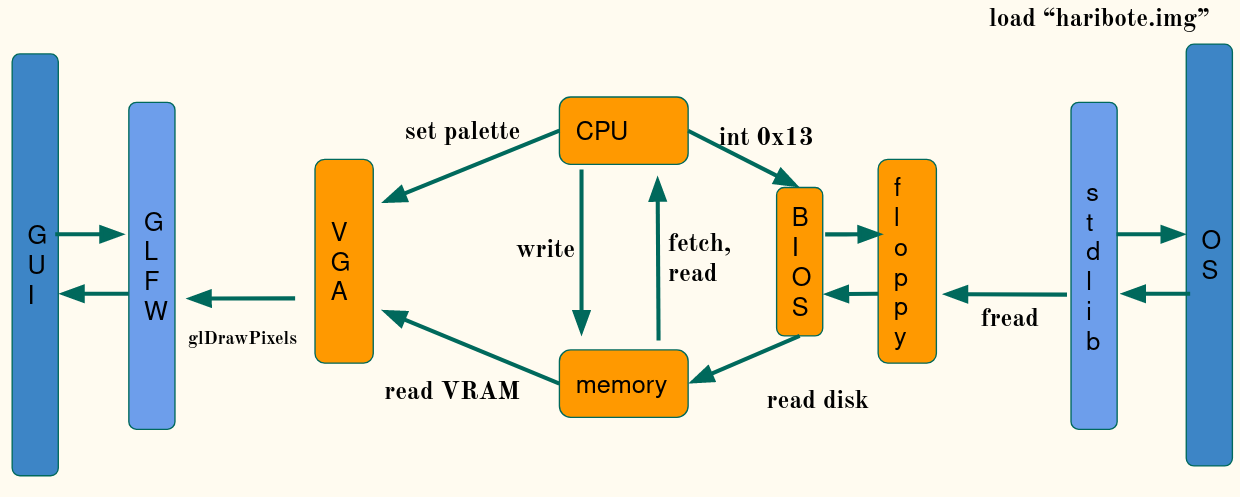
\includegraphics[width=7.5cm]{./emu_struct.png}
		\caption{自作エミュレータの構造}
		\label{emustruct}
	\end{center}
\end{figure}

\section{実装}
EmscriptenはWebAssembly向けのコンパイラだけではなく,
標準ライブラリやOpenGLなどの一部のライブラリをJavaScriptに移植したものを含んでいる.
そのため,それらのライブラリのみを使用したアプリケーションはC/C++のコンパイラを"emcc"に指定するだけでブラウザ向けにビルドすることができる.

しかし,それだけでは自作のエミュレータを移植することはできなかった.
これにより移植できたのは図\ref{emustruct}の中央のオレンジ色で示した部分にとどまった.

\subsection{ファイル読み込み}
移植できなかった部分のうち,
図\ref{emustruct}の右側のファイル読み込みについては,
Emscriptenに対して読み込むファイルの指定をすることで,
fread関数を呼ぶだけでフォントファイル\footnote{VGAテキストモードのエミュレーション時に用いるフォント.}
とフロッピーディスクのイメージファイルを問題無く読み込むことができた.

これにより,"emu.data"のようなバイナリファイルが生成される.
ファイルアクセス時には,このファイルに対してJavaScriptのFileSystem APIを用いてアクセスし,
Emscriptenの標準ライブラリにファイルのバイナリイメージが渡されることによって実現されている.

\subsection{画面描画}
% pthreadがexperimental
% glDrawPixelsが使えない
% emscripten_loopが使えない
% 最終的にやったこと

次に取り組んだのが図\ref{emustruct}の左側の,画面描画部分の移植となる.

自作エミュレータでの画面描画のエミュレーションは以下のような手順を踏んで行われている.

\begin{enumerate}
	\item paletteの設定(out命令により行われる)
	\item VRAMの読み込み
	\item RGBデータの生成
	\item glDrawPixels()によりウィンドウに表示
\end{enumerate}

これらのうち,1以外はメインスレッドとは別のスレッドで実行される操作となっている.
しかし,WebAssemblyにおけるpthread実装はまだproposalの段階であったため,
定期的に2〜4の操作をメインスレッドで行うことで描画を行うことを考えた.
だが,glDrawPixelsというOpenGLの関数がWebGLでサポートされていなかった
\footnote{glDrawPixelsはOpenGL ES 2.0で削除された関数であり,WebGLはこの規格に相当するAPIを提供している.}
他,main関数の実行中に描画(正確にはDOMへの操作)を更新するために必要なemscripten\_sleepというEmscriptenの関数をソースコード中に入れるとコンパイラが落ちる
\footnote{コンパイルエラーではなく,コンパイラ中で何らかのassertが失敗しているようだったのだが,小さなプログラムでは再現しなかったため詳しい原因はよく分かっていない.}
,といった問題があり,中々描画を行うことができなかった.

そのため,main関数実行中の描画は諦め,
エミュレーション終了時の画面の状態を描画することとし,
RGBデータの描画はEM\_ASM\_というマクロを用いてmain関数から直接canvasに書き込むことで行うことにした.

\begin{figure}[htbp]
	\begin{center}
		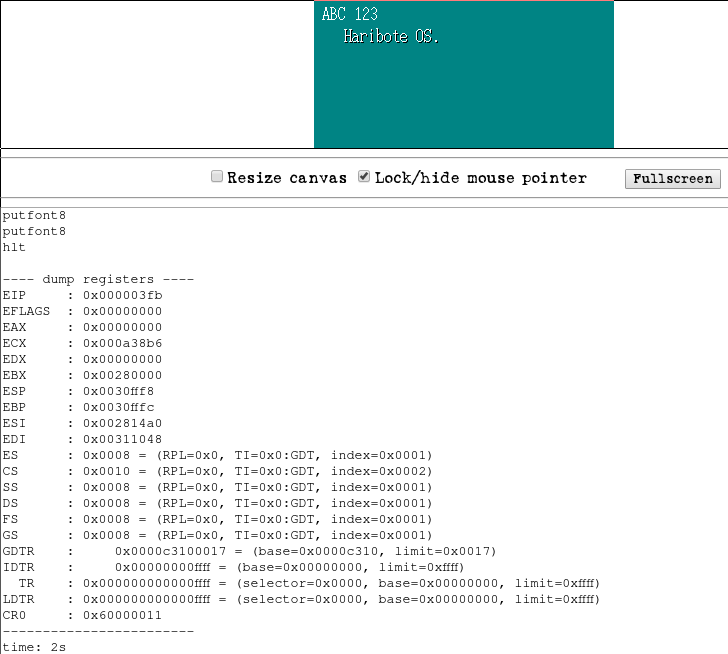
\includegraphics[width=8cm]{./demo.png}
		\caption{実行の様子}
		\label{demo}
	\end{center}
\end{figure}

最終的に,図\ref{demo}のようにcanvasに対してエミュレーション終了時のVGAの描画データを書き込み,表示することができた.

\section{まとめ}
Emscriptenを用いることで,
自作のエミュレータをコア部分を変更することなくブラウザに移植できることが分かった.
また,

今回は自作のエミュレータが動作するプラットフォームを増やすことを目的にこのような移植を行った.
しかし,このエミュレータを開発した元々の目的は,
普段何気なく使用しているコンピュータの動作原理を学ぶためであった.
今期もそのために,FreeDOSを動作させることを目標として新規にエミュレータを開発する予定だったのだが,
実装のための時間を中々作ることができなかったため,今回の発表はこのような形となった.

そのため,来期以降は自作エミュレータへのメモリ保護機構やキーボード入力の実装や,
FPGAでCPUを自作することで更に下のレイヤからコンピュータの動作原理を学ぶ,といったことを行いたいと考えている.

\bibliographystyle{junsrt}
\bibliography{resume}

\end{document}
% end of file
